\documentclass[../thesis.tex]{subfiles}
\begin{document}
\chapter{Performance Analysis}\label{cap:performance_analysis}

This chapter describes the tests carried out to evaluate the effectiveness of the different web crawler implementations deployed for this thesis. The first section introduces the monitoring stack that allowed the gathering, visualization and storage of the metrics needed to compare the performance of the proposed architectures. The second section illustrates these tests, the motivation behind the choice of target \acrshort{URL} and the cluster configuration for each variant. Finally, the results are reported in the last section and significant plots are shown.

\section{Monitoring Stack}
The usage of auxiliary technologies was necessary to collect, visualize and store the metrics exposed during the test executions. For these reasons, we based our monitoring stack on well-known tools such as Prometheus Stack \cite{site:kube_prom_stack}, InfluxDB \cite{site:influxdb}, Telegraf \cite{site:telegraf} and CloudWatch \cite{site:cloudwatch_doc}, which was provided by \acrshort{AWS} and only useful for the implementation that exploits Lambda service. All other tools are open-source and have been deployed using \gls{helm_chart}s.

\texttt{Prometheus Stack}, also known as \texttt{kube-prometheus stack}, is a collection of Kubernetes manifests, Grafana dashboards and Prometheus rules, as well as documentation and scripts, which enables easy end-to-end monitoring of the \gls{k8s} cluster using \textit{Prometheus Operator}.

\begin{itemize}
    \item \textit{Prometheus} is the heart of the stack and provides a monitoring platform that collects metrics from the monitored targets by scraping the \acrshort{HTTP} endpoints made available on those targets;
    \item \textit{Grafana} enables the analysis and visualization of metrics from various sources, including databases, applications and monitoring systems such as Prometheus;
    \item \textit{kube-state-metrics} listens to the \gls{k8s} \acrshort{API} server and generates metrics about the state of the objects (e.g. \gls{deployment}s, \gls{pod}s, \gls{job}s, etc.);
    \item Other components included in the stack but not useful for our tests are \textit{node-exporter} and \textit{Alertmanager}.
\end{itemize}

\texttt{InfluxDB} is a time series database designed to handle high write and query loads for efficient monitoring and analysis of time data such as metrics and events.

\texttt{Telegraf} is a plugin-driven server agent used to collect metrics from various sources and then send this data to various data stores or visualization platforms for monitoring and analysis.

\texttt{CloudWatch} is an \acrshort{AWS} service that monitors and collects real-time metrics, log files, and events from \acrshort{AWS} resources and on-premises servers. It enables users to set alarms, analyze data and create custom dashboards.

\autoref{fig:architecture_monitoring} shows both architectures used by the different cloud providers.

\begin{figure}[H]
\centering
    \begin{subfigure}[b]{.75\textwidth}
        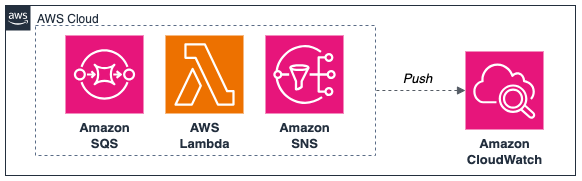
\includegraphics[width=.94\textwidth]{performance_analysis/architecture_monitoring_aws.png}
        \caption[Monitoring stack architecture on \acrshort{AWS}]{On \acrshort{AWS}.}
        \label{fig:architecture_monitoring_aws}
    \end{subfigure}
    \begin{subfigure}[b]{1\textwidth}
        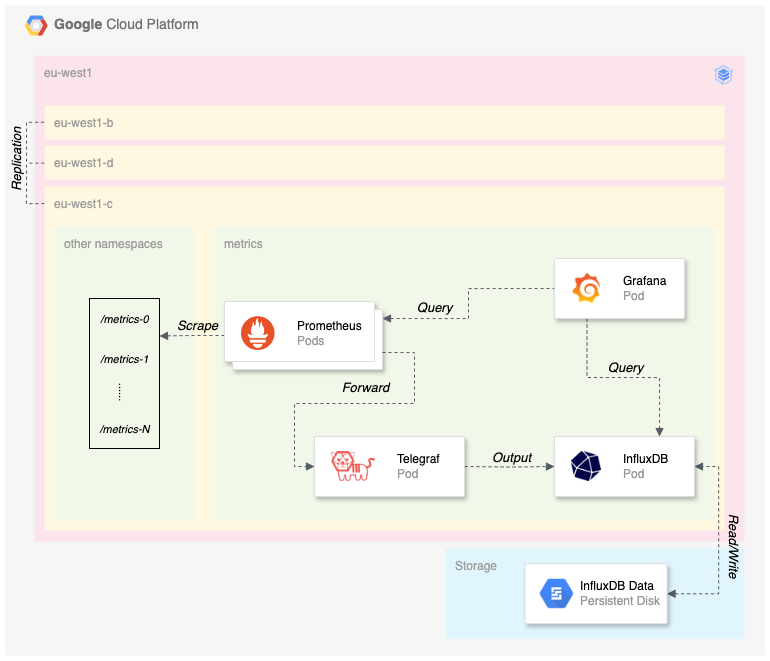
\includegraphics[width=1\textwidth]{performance_analysis/architecture_monitoring_gke.png}
        \caption[Monitoring stack architecture on \acrshort{GKE}]{On \acrshort{GKE}.}
        \label{fig:architecture_monitoring_gke}
    \end{subfigure}
\caption{Monitoring stack architectures.}
\label{fig:architecture_monitoring}
\end{figure}

Regarding \acrshort{AWS} (\autoref{fig:architecture_monitoring_aws}), using CloudWatch doesn't require configurations; the services employed automatically send metrics to it. We had only to familiarise ourselves with the \acrshort{UI} to easily view pre-defined dashboards based on the selected service and download data points in \acrshort{CSV} format.

Instead, several steps were required to configure the chosen monitoring system on \acrshort{GKE}. The two guides provided by Knative \cite{site:knative_collecting_metrics} and InfluxData \cite{site:prom_tel_influx} were followed and the setup configurations were reported on \autoref{appendix:monitoring_conf}. Summarizing, Prometheus collects all metrics from the monitored targets and forwards them to Telegraf using the \texttt{remote\_write} \acrshort{API}. Telegraf receives input metrics every 10 seconds and sends them as output to the designated bucket on InfluxDB for permanent storage. This allows us to analyse saved time series data directly from InfluxDB using the Flux\footnote{Flux is InfluxData’s functional data scripting language designed for querying, analyzing, and acting on data. See \href{https://docs.influxdata.com/influxdb/cloud/query-data/get-started/}{https://docs.influxdata.com/influxdb/cloud/query-data/get-started/} for more details.} language. Alternatively, we can use Grafana, which provides pre-configured dashboards for \gls{k8s}, Knative and RabbitMQ.

\section{Test Design}
The test suite aims to analyse the performance of the three implementations, considering both the available web crawling methods, \acrshort{HTTP} requests and browser automation. For every one of the six test configurations, we will vary the \textit{maxVisitedUrls} parameter across values of $[250, 1000, 4000]$, determining the maximum number of web pages to be visited by the crawler. 

Eighteen executions in total will therefore be carried out, each of which will be repeated only once, due to the high cost of the infrastructure for the Knative-based implementation.

The target \acrshort{URL} chosen to run these tests was \href{https://apkpure.net/it/}{https://apkpure.net/it/}, a website where you can download open-source Android applications that, however, does not have strict verification procedures like Google Play and could therefore contain malware. ApkPure is legal, but sometimes it's possible that the platform may host unauthorized content like cracked or pirated apps, meaning there is a risk of encountering illegal material if you decide to explore it \cite{site:nordvpn_apkpure, site:avast_apkpure}. For this reason, it could be a specific use case for the application presented in this thesis.

\subsection{Metrics}
In all test configurations, the following metrics were considered:

\begin{itemize}
    \item search \textbf{duration} (time between the start of a search and its completion with the last result, in the format \textit{hh:mm:ss,ms})
    \item cumulative \textbf{size of messages} in bytes (amount of data handled during communications)
    \item cumulative \textbf{error count}
\end{itemize}

\subsection{Cluster configurations}
In order to execute the tests, we first set up the cluster for the \acrshort{AWS} implementation. A three-node cluster was created on \acrshort{GKE} with 6 vCPUs and 20 GB of memory, necessary to deploy the monitoring stack, Elasticsearch cluster and the backend's \gls{deployment}s.

The second implementation based on \gls{k8s} used the same cluster; the backend's \gls{deployment}s were updated and the necessary manifests to authenticate the \gls{k8s} client were added. There was no need to increase resources because only one search was carried out at a time.

The final implementation, using Knative, required more resources due to the additional components and the need to provide 100 concurrent functions. For these reasons, a new pool of three nodes with 92 vCPU and 384GB of memory was created to replace the previous one.

\section{Experimental Results}
The following sections contain the results of the different implementations. A table and a plot will be shown for the first two metrics, search duration and cumulative size of messages.  Instead, the third metric will only be shown through a plot.

All of them require the rental of a cluster via a cloud provider, but the difference in resources required for Knative, compared to the managed version that follows the same serverless paradigm, provided by \acrshort{AWS} Lambda, is considerable.

\newpage

\autoref{fig:plot_duration_http_request} illustrates the search duration of each configuration. We can notice an increase in times as more \acrshort{URL}s are visited, the Knative implementation is the one that performed best, followed by \acrshort{AWS} and finally \gls{k8s}. These results were expected as the serverless paradigm is more performance-oriented due to more concurrent executions, with Knative having the advantage over \acrshort{AWS} due to the ability to manage autoscaling as desired, as well as not having to communicate with services outside the cluster (e.g. \acrshort{SQS}, \acrshort{SNS}).

\vspace*{4cm}

\begin{figure}[H]
    \centering
    % Duration HTTP
    %\captionof{table}{A table}\label{tab:atable}
    \begin{tabular}{|c|c|c|c|}
        \hline
        \multicolumn{4}{|c|}{\textbf{HTTP Request}} \\
        \hline
        & \multicolumn{3}{c|}{\textit{\textbf{Implementations}}} \\
        \hline
        \textit{\textbf{Num. URLs}} & \multicolumn{1}{c|}{\textit{Knative}} & \multicolumn{1}{c|}{\textit{AWS}} & \multicolumn{1}{c|}{\textit{Kubernetes}} \\
        \hline
        \textit{250} & 00:00:20,103 & 00:02:44,066 & 00:01:04,241 \\
        \hline
        \textit{1000} & 00:00:39,495 & 00:02:03,878 & 00:04:34,639 \\
        \hline
        \textit{4000} & 00:02:02,620 & 00:05:33,763 & 00:14:45,958 \\
        \hline
    \end{tabular}
    
    \vspace{\floatsep}

    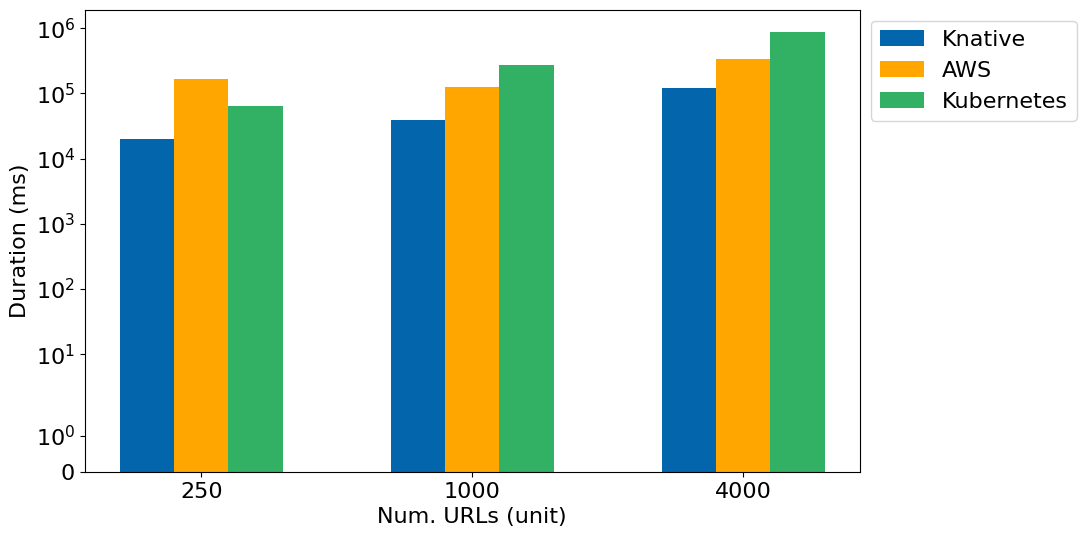
\includegraphics[width=1\textwidth]{performance_analysis/plot_duration_http_request.png}

    \captionof{figure}[Results on search duration - HTTP]{Results on search duration with \acrshort{HTTP} request method.}\label{fig:plot_duration_http_request}
\end{figure}

\newpage

\autoref{fig:plot_duration_pptr} shows the same trend as before, with obviously longer duration due to browser management. It is interesting to notice the last \gls{k8s} test with 4000 \acrshort{URL}s, which reached a duration of over 4 hours. This could be due to using the same browser for a large number of web pages.

\vspace*{5cm}

\begin{figure}[H]
    \centering
    % Duration PPTR
    \begin{tabular}{|c|c|c|c|}
        \hline
        \multicolumn{4}{|c|}{\textbf{Browser Automation}} \\
        \hline
        & \multicolumn{3}{c|}{\textit{\textbf{Implementations}}} \\
        \hline
        \textit{\textbf{Num. URLs}} & \multicolumn{1}{c|}{\textit{Knative}} & \multicolumn{1}{c|}{\textit{AWS}} & \multicolumn{1}{c|}{\textit{Kubernetes}} \\
        \hline
        \textit{250} & 00:01:42,815 & 00:04:35,153 & 00:14:41,554 \\
        \hline
        \textit{1000} & 00:03:13,657 & 00:06:02,608 & 00:59:49,047 \\
        \hline
        \textit{4000}  & 00:08:08,082 & 00:10:39,026 & 04:10:34,170 \\
        \hline
    \end{tabular}
    
    \vspace{\floatsep}

    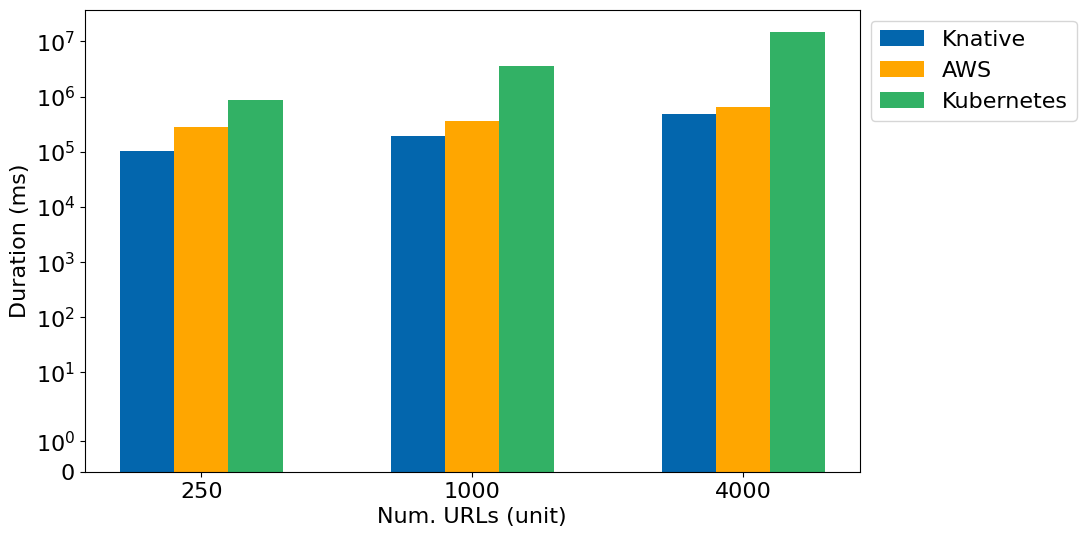
\includegraphics[width=1\textwidth]{performance_analysis/plot_duration_pptr.png}

    \captionof{figure}[Results on search duration - Browser]{Results on search duration with Browser Automation method.}\label{fig:plot_duration_pptr}
\end{figure}

\newpage

\autoref{fig:plot_size_msg_http} displays the results of the cumulative \textbf{size of messages} metric. As we saw in the previous chapter, the \gls{k8s} implementation does not exploit any queuing or notification mechanism, so we tracked the size of the response object that the client used to create a \gls{job}. It is invariant across the different numbers of \acrshort{URL}s because it is taken directly from the database; we submitted the same object with the same environment variables. For these reasons, it is the implementation with the lowest value. AWS and Knative have similar results, with the latter remaining slightly lower but tending to increase probably for two reasons:

\begin{itemize}
    \item the overhead generated by the return messages of the various functions, used for logging purposes;
    \item The higher throughput of \acrshort{HTTP} requests compared to browser automation causes more CloudEvents to contain less than five \acrshort{URL}s, as the requests do not get queued up. This increases the amount of messages sent when using \acrshort{HTTP} request, while having no effect when using browser automation.
\end{itemize}

\vspace*{2cm}

\begin{figure}[H]
    \centering
    % Size of messages HTTP
    \begin{tabular}{|c|c|c|c|}
        \hline
        \multicolumn{4}{|c|}{\textbf{HTTP Request}} \\
        \hline
        & \multicolumn{3}{c|}{\textit{\textbf{Implementations}}} \\
        \hline
        \textit{\textbf{Num. URLs}} & \multicolumn{1}{c|}{\textit{Knative}} & \multicolumn{1}{c|}{\textit{AWS}} & \multicolumn{1}{c|}{\textit{Kubernetes}} \\
        \hline
        \textit{250} & 49052 & 1642277 & 7708 \\
        \hline
        \textit{1000} & 3571312 & 7080464 & 7708 \\
        \hline
        \textit{4000}  & 67007627 & 32316143 & 7708 \\
        \hline
    \end{tabular}
    
    \vspace{\floatsep}

    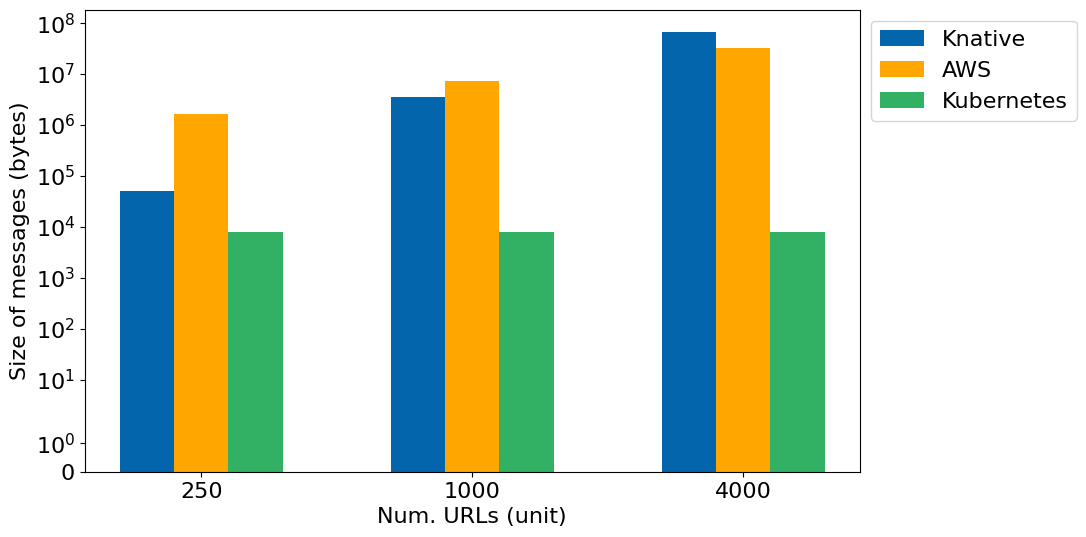
\includegraphics[width=1\textwidth]{performance_analysis/plot_size_msg_http.png}

    \captionof{figure}[Results on size of messages - HTTP]{Results on cumulative size of messages with \acrshort{HTTP} request method.}\label{fig:plot_size_msg_http}
\end{figure}

\newpage

\autoref{fig:plot_size_msg_pptr} follows a similar pattern, the Knative implementation using the browser method can better manage the number of requests stored within each CloudEvents, which is why we have lower values than the other method.

\vspace*{5cm}

\begin{figure}[H]
    \centering
    % Size of messages PPTR
    \begin{tabular}{|c|c|c|c|}
        \hline
        \multicolumn{4}{|c|}{\textbf{Browser Automation}} \\
        \hline
        & \multicolumn{3}{c|}{\textit{\textbf{Implementations}}} \\
        \hline
        \textit{\textbf{Num. URLs}} & \multicolumn{1}{c|}{\textit{Knative}} & \multicolumn{1}{c|}{\textit{AWS}} & \multicolumn{1}{c|}{\textit{Kubernetes}} \\
        \hline
        \textit{250} & 101059 & 1782075 & 7708 \\
        \hline
        \textit{1000} & 678352 & 8624444 & 7708 \\
        \hline
        \textit{4000}  & 7755194 & 28512443 & 7708 \\
        \hline
    \end{tabular}
    
    \vspace{\floatsep}

    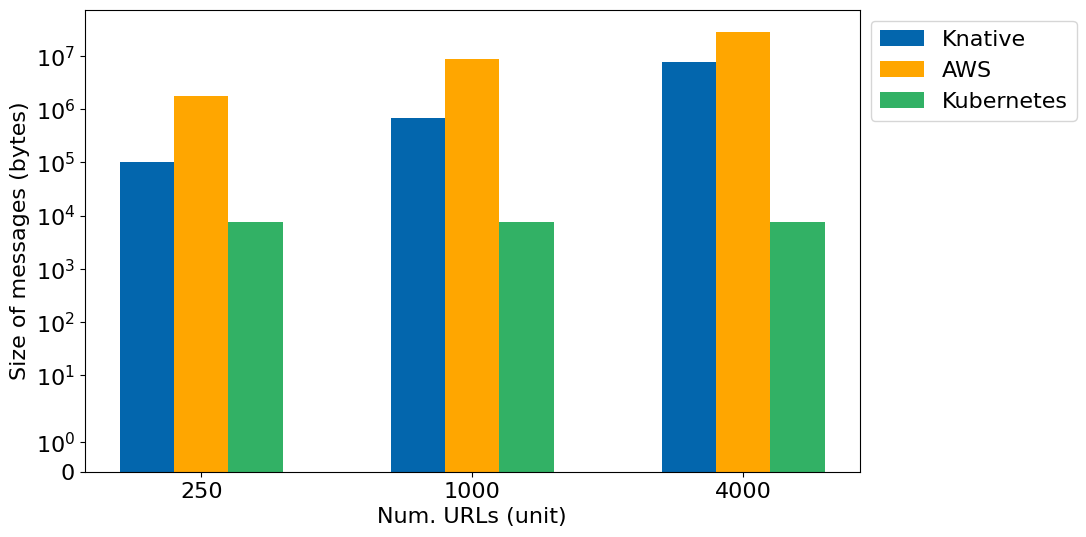
\includegraphics[width=1\textwidth]{performance_analysis/plot_size_msg_pptr.png}

    \captionof{figure}[Results on size of messages - Browser]{Results on cumulative size of messages with Browser Automation method.}\label{fig:plot_size_msg_pptr}
\end{figure}

\newpage

Finally, in \autoref{fig:plot_errors_http_request} and \ref{fig:plot_errors_pptr}, it can be seen that only the \acrshort{AWS} implementation reported errors during testing. This could be due to the timeout set to 60s on the Lambda or some rate limit implementing the visited website for the \acrshort{AWS} \acrshort{IP}s.

\vspace*{3cm}

\begin{figure}[H]
    \centering
    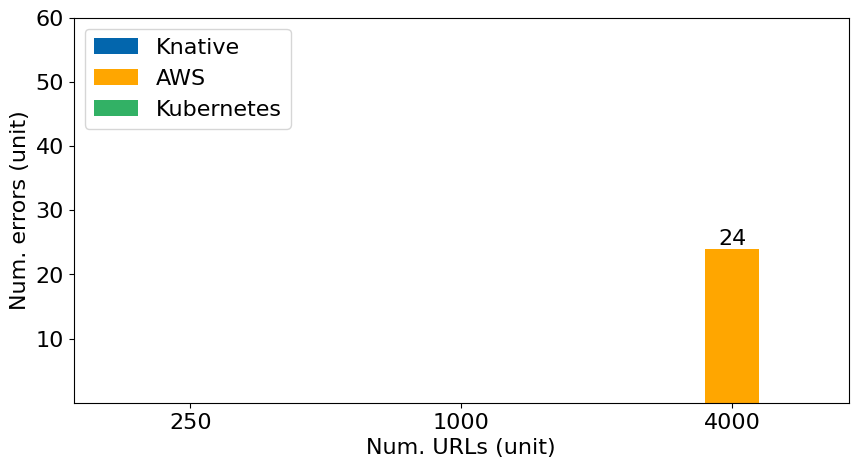
\includegraphics[width=.85\textwidth]{performance_analysis/plot_errors_http_request.png}
    \caption[Results on error count - HTTP]{Results on error count with \acrshort{HTTP} request method.}\label{fig:plot_errors_http_request}
\end{figure}

\begin{figure}[H]
    \centering
    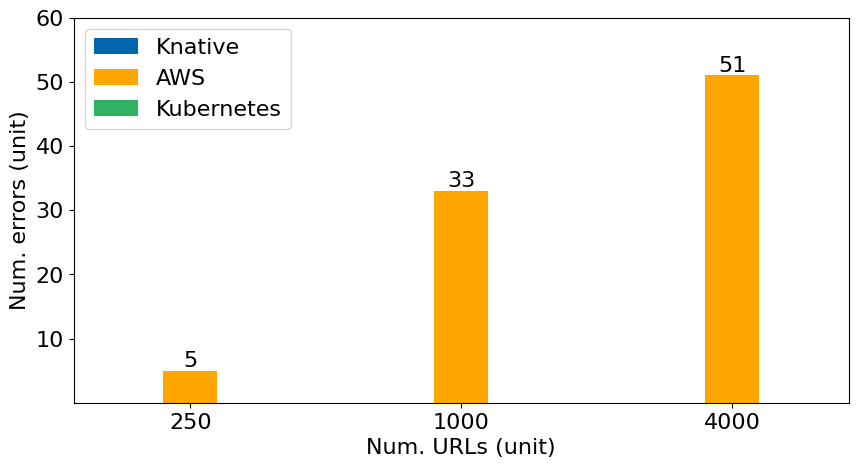
\includegraphics[width=.85\textwidth]{performance_analysis/plot_errors_pptr.png}
    \caption[Results on error count - Browser]{Results on error count with Browser Automation method.}\label{fig:plot_errors_pptr}
\end{figure}

\end{document}